\documentclass{harvardml}

% Authors: Amir Shanehsazzadeh, Andrew Kim, Nari Johnson (Jan 2021)
% Edited by: Max Guo, Raphael Pellegrin, Katherine Tian (Jan 2022)
% Edited once more by: William Tong (Jan 2023), Skyler Wu (Jan 2023)

% Adapted from CS281 Fall 2019 section 0 notes

% This tex file relies on
% the presence of two files:
% harvardml.cls and common.sty

\course{CS181-s23}
\assignment{Homework \#0}
\duedate{January 26, 2023 at 11:59 PM\\ (with free, no-questions-asked extension, see below)}

\usepackage{comment}
\usepackage{url}
\usepackage{graphicx}
\usepackage{amsfonts, amsmath, amsthm}
\usepackage{listings}
\usepackage[shortlabels]{enumitem}
\usepackage{hyperref}

\theoremstyle{definition}
\newtheorem{defn}{Definition}[section]
\theoremstyle{plain}
\usepackage[textsize=tiny]{todonotes}

% Some useful macros.
\newcommand{\given}{\,|\,}
\newcommand{\R}{\mathbb{R}}
\newcommand{\C}{\mathbb{C}}
\newcommand{\E}{\mathbb{E}}
\newcommand{\var}{\text{Var}}
\newcommand{\cov}{\text{Cov}}
\newcommand{\p}{\partial}
\newcommand{\mba}{\mathbf{a}}
\newcommand{\mbb}{\mathbf{b}}
\newcommand{\mbx}{\mathbf{x}}
\newcommand{\mcX}{\mathcal{X}}
\newcommand{\mcY}{\mathcal{Y}}
\newcommand{\boldw}{\mathbf{w}}
\newcommand{\mbxt}{\tilde{\mathbf{x}}}
\newcommand{\Sigmat}{\tilde{\Sigma}}
\newcommand{\mbz}{\mathbf{z}}
\newcommand{\mbw}{\mathbf{w}}
\newcommand{\mcN}{\mathcal{N}}
\newcommand{\mcP}{\mathcal{P}}
\newcommand{\eps}{\epsilon}
\newcommand{\trans}{\intercal}
\newcommand{\Ut}{\tilde{U}}
\DeclareMathOperator*{\argmax}{arg\,max}
\newcommand{\angstrom}{\textup{\AA}}
\renewcommand{\v}[1]{\mathbf{#1}}


\usepackage{xcolor}
\newcount\Comments  % 0 suppresses notes to selves in text
\Comments = 1
\newcommand{\kibitz}[2]{\ifnum\Comments=1{\color{#1}{#2}}\fi}
\newcommand{\dcp}[1]{\kibitz{blue}{[DCP: #1]}}

\begin{document}

\noindent Welcome to CS181! The purpose of this assignment is to help assess your readiness for this course. \textbf{This assignment will be graded for completion and effort.} If you encounter any difficulty with these problems, fear not! We will have sections in the first week of class reviewing the math, statistics, and coding pre-requisites for this course. TFs will also directly discuss relevant problems from this HW0 in these sections. You are, of course, more than welcome to swing by office hours and post questions on Ed.

\begin{enumerate}
    \item Please type your solutions after the corresponding problems using this \LaTeX\ template, and start each problem on a new page.
    \item Please submit the \textbf{writeup PDF to the Gradescope assignment `HW0'}. Remember to assign pages for each question.
    \item Please submit your \textbf{\LaTeX\ file and code files (i.e., anything ending in \texttt{.py}, \texttt{.ipynb}, or \texttt{.tex}) to the Gradescope assignment `HW0 - Supplemental'}. 
\end{enumerate}

\noindent \textbf{Free, No-Questions-Asked Extension:}
\begin{itemize}
    \item The official deadline is January 26, in order to not overlap too much with HW1, which covers substantial new course material. With teaching staff discussing these problems in Week 1 sections, a reasonably prepared (in terms of pre-requisites) student should be able to complete this assignment quite comfortably in a week.
    \item However, given the uncertainty and frenzy of the start of the new semester, we will also give free, no-questions-asked extensions to \textbf{February 2, 2023 at 11:59 PM} if you need some extra breathing room and / or if you need to brush up a little more on the pre-requisites. Do note, however, that HW1 will be due a week later on February 9.
    \item You do not need to formally request this free, no-questions-asked extension (i.e., no Ed post or email is necessary). Please simply submit your assignment before the late deadline of \textbf{February 2, 2023 at 11:59 PM} in Gradescope. Given that this is a free extension, it does not count into your late days for the semester.
\end{itemize}


\begin{problem}[Modeling Linear Trends - Linear Algebra Review]
In this class we will be exploring the question of ``how do we model the trend in a dataset" under different guises. In this problem, we will explore the algebra of modeling a linear trend in data. We call the process of finding a model that capture the trend in the data, ``fitting the model."\\

\noindent \textbf{Learning Goals:} In this problem, you will practice translating machine learning goals (``modeling trends in data") into mathematical formalism using linear algebra. You will explore how the right mathematical formalization can help us express our modeling ideas unambiguously and provide ways for us to analyze different pathways to meeting our machine learning goals.\\

\noindent Let's consider a dataset consisting of two points $\mathcal{D} = \{(x_1, y_1), (x_2, y_2)\}$, where $x_n, y_n$ are scalars for $n=1, 2$. Recall that the equation of a line in 2-dimensions can be written: $y = w_0 + w_1x$. 
\begin{enumerate}
    \item Write a system of linear equations determining the coefficients $w_0, w_1$ of the line passing through the points in our dataset $\mathcal{D}$ and analytically solve for $w_0, w_1$ by solving this system of linear equations (i.e., using substitution). Please show your work.
    \item Write the above system of linear equations in matrix notation, so that you have a matrix equation of the form $\mathbf{y} = \mathbf{X}\mathbf{w}$, where $\mathbf{y}, \mathbf{w} \in \mathbb{R}^2$ and $\mathbf{X} \in \mathbb{R}^{2\times 2}$. For full credit, it suffices to write out what $\mathbf{X}$, $\mathbf{y}$, and $\mathbf{w}$ should look like in terms of $x_1$, $x_2$, $y_1$, $y_2$, $w_0$, $w_1$, and any other necessary constants. Please show your reasoning and supporting intermediate steps.
    \item Using properties of matrices, characterize exactly when a unique solution for $\mathbf{w}=\left(w_0 \; w_1 \right)^{T}$ exists. In other words, what must be true about your dataset in order for there to be a unique solution for $\mathbf{w}$? When the solution for $\mathbf{w}$ exists (and is unique), write out, as a matrix expression, its analytical form (i.e., write $\mathbf{w}$ in terms of $\mathbf{X}$ and $\mathbf{y}$).
    
    Hint: What special property must our $\mathbf{X}$ matrix possess? What must be true about our data points in $\mathcal{D}$ for this special property to hold?
    \item Compute $\mathbf{w}$ by hand via your matrix expression in (3) and compare it with your solution in (1). Do your final answers match? What is one advantage for phrasing the problem of fitting the model in terms of matrix notation? 
    \item In real-life, we often work with datasets that consist of hundreds, if not millions, of points. In such cases, does our analytical expression for $\mathbf{w}$ that we derived in (3) apply immediately to the case when $\mathcal{D}$ consists of more than two points? Why or why not?
\end{enumerate}    
\end{problem}
\newpage
\begin{enumerate}
    \item $y_1 = w_0 + w_1x_1$ and $y_2 = w_0 + w_1x_2$ implies, substituting $w_0$, 
    $$
    w_0 = y_2 - w_1x_2 \implies y_1 = y_2 - w_1x_2 + w_1x_1 \implies y_1 - y_2 = w_1(x_1 - x_2)
    $$
    So, 
    $$
    \frac{y_1 - y_2}{x_1 - x_2} = w_1
    $$
    Plugging this into the first equation, we have
    $$
    y_1 = w_0 + \frac{x_1(y_1 - y_2)}{x_1 - x_2} \implies w_0 = y_1 - \frac{x_1(y_1 - y_2)}{x_1 - x_2}
    $$
    \item We can write $\vec{w}$ and $\vec{y}$ as the following vectors:
    $$
    \begin{bmatrix}
        w_0 \\ w_1
    \end{bmatrix}
    \begin{bmatrix}
        y_1 \\ y_2
    \end{bmatrix}
    $$
    Since we're solving for the values of $w_0$ and $w_1$, we want our augmented matrix to contain no values in terms of $w_n$ (we don't want to define $w_n$ in terms of itself). Thus, we can write $X$ as the following matrix
    $$
    \begin{bmatrix}
        1 & x_1 \\ 1 & x_2
    \end{bmatrix}$$
    We use the values 1 and $x_1$ because we want the equation to be such that we get $w_0 + w_1x_1$. When we multiply each column by $\mathbf{w}$, we get these values when each row is of the form $\begin{bmatrix}
        1 & x_n
    \end{bmatrix}$
    \item By the Invertible Matrix Theorem, there exists a unique solution for $\mathbf{w}$ whenever $\mathbf{X}$ is invertible. The inverse of $\mathbf{X}$ is 
    $$
    \begin{bmatrix}
    \frac{x_2}{x_2-x_1}&-\frac{x_1}{x_2-x_1}\\
    -\frac{1}{x_2-x_1}&\frac{1}{x_2-x_1}
    \end{bmatrix}
    $$
    We can see, then, that $\mathbf{X}$ is invertible if and only if $x_1 \neq x_2$. This makes sense: if $x_1 = x_2$, we only have one $x$-value, and we cannot draw a line between two points: we either have a solution of all real numbers or no solution.
    \item We can find $\mathbf{w}$ by turning it into reduced-row echelon form. First, we augment $\mathbf{X}$ by $\mathbf{y}$. Then, we get 
    $$
    \begin{bmatrix}
    1&0&\frac{-x_1y_2+y_1x_2}{x_2-x_1}\\ 
    0&1&\frac{y_2-y_1}{x_2-x_1}
    \end{bmatrix}
    $$
    $w_1 = \frac{y_2-y_1}{x_2-x_1} = \frac{y_1-y_2}{x_1-x_2}$ is equivalent in both cases, since the positive or negative sign will hold: if $x$ and $y$ positively correlate, then, assuming $y_2 > y_1$ and $x_2 > x_1$, both expression will be greater than zero. Assuming the same thing, and that $x$ and $y$ negatively correlate, both expressions will be less than zero. If there is no correlation (i.e., the line graphing $x_n$ and $y_n$ is flat), then the numerator will be zero. 
    \newline $w_1$ is also equivalent: we can get a common denominator for part 1)'s version of $w_1: y_1 - \frac{x_1(y_1 - y_2)}{x_1 - x_2} = \frac{y_1(x_1 - x_2)}{x_1 - x_2} - \frac{x_1(y_1 - y_2)}{x_1 - x_2} = \frac{y_1x_1 - y_1x_2)}{x_1 - x_2} - \frac{x_1y_1 - x_1y_2}{x_1 - x_2} = \frac{x_1y_2 - y_1x_2)}{x_1 - x_2}$, which is equivalent to the value derived in the matrix for the same reason as above. 
    \item If $\mathcal{D}$ is a perfectly linear dataset, then the expressions we derive for the coefficients do hold, but this is rarely the case; usually we will have to approximate the datapoints. 
\end{enumerate}



\begin{problem}[Optimizing Objectives - Calculus Review]
In this class, we will write real-life goals we want our model to achieve into a mathematical expression and then find the optimal settings of the model that achieves these goals. The formal framework we will employ is that of mathematical optimization. Although the mathematics of optimization can be quite complex and deep, we have all encountered basic optimization problems in our first calculus class!\\

\noindent \textbf{Learning Goals:} In this problem, we will explore how to formalize real-life goals as mathematical optimization problems. We will also investigate under what conditions these optimization problems have solutions.\\

\noindent In her most recent work-from-home shopping spree, Nari decided to buy several house plants. \textit{Her goal is to make them to grow as tall as possible.} After perusing the internet, Nari learns that the height $y$ in mm of her Weeping Fig plant can be directly modeled as a function of the oz of water $x$ she gives it each week:
$$y = - 3x^2 + 72x + 70.$$
\begin{enumerate}
    \item Based on the above formula, is Nari's goal achievable: does the plant have a maximum height? Why or why not? Does her goal have a unique solution - i.e. is there one special watering schedule that would acheive the maximum height (if it exists)?
    
    Hint: plot this function. In your solution, words like ``convex" and ``concave" may be helpful.
    \item Using calculus, find how many oz per week should Nari water her plant in order to maximize its height. With this much water, how tall will her plant grow?

    Hint: solve analytically for the critical points of the height function (i.e., where the derivative of the function is zero).  For each critical point, use the second-derivative test to identify if each point is a  max or min point, and use arguments about the global structure (e.g., concavity or convexity) of the function to argue whether this is a local or global optimum.
\end{enumerate}
Now suppose that Nari want to optimize both the amount of water $x_1$ (in oz) \textit{and} the amount of direct sunlight $x_2$ (in hours) to provide for her plants. After extensive research, she decided that the height $y$ (in mm) of her plants can be modeled as a two variable function:

$$y = f(x_1, x_2) = \exp\left(-(x_1 - 2)^2 - (x_2 - 1)^2 \right)$$
\begin{enumerate}
    \setcounter{enumi}{2}
    \item Using \texttt{matplotlib}, visualize in 3D the height function as a function of $x_1$ and $x_2$ using the \texttt{plot\_surface} utility for $(x_1, x_2) \in (0, 6) \times (0, 6)$. Use this visualization to argue why there exists a unique solution to Nari's optimization problem on the specified intervals for $x_1$ and $x_2$.

    Remark: in this class, we will learn about under what conditions do \textit{multivariate} optimization problems have unique global optima (and no, the second derivative test doesn't exactly generalize directly). Looking at the visualization you produced and the expression for $f(x_1, x_2)$, do you have any ideas for why this problem is guaranteed to have a global maxima? You do not need to write anything responding to this -- this is simply food for thought and a preview for the semester.
\end{enumerate}

\end{problem}

\newpage
\begin{enumerate}
    \item Nari's plant does have a maximum height; it is 502mm. We can find this by plotting it; in this case, the graph is concave down--an upside-down parabola. We can also find it by setting the derivative equal to zero and noting that it is concave.  
    \item We can find this by first finding the first derivative of the equation:
    $$
    f(x) = - 3x^2 + 72x + 70 \implies 0 = f'(x) = -6x + 72 \implies x = 12
    $$
    The second derivative is $f''(x) = -6 < 0$ for all $x$, so the equation is always concave down (which we know is true from the graph). Because the graph is always concave down, this must be a maximum. From the above, we know that the first derivative can only be zero at one value, so this is the only maximum of a concave down equation, and thus the global maximum.    
    \item 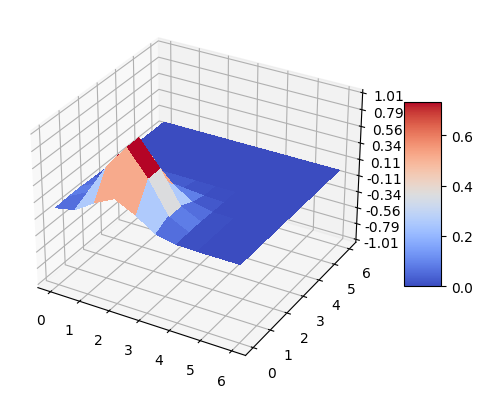
\includegraphics{hw0/height_graph.png} \newline
    In the above image, we can see that there is a single maximum of plant height, and it is decreasing around that maximum of (1, 3) (I derived that in the code). 
\end{enumerate}

\begin{problem}[Reasoning about Randomness - Probability and Statistics Review]
In this class, one of our main focuses is to model the unexpected variations in real-life phenomena using the formalism of random variables. In this problem, we will use random variables to model how much time it takes an USPS package processing system to process packages that arrive in a day.\\

\noindent \textbf{Learning Goals:} In this problem, you will analyze random variables and their distributions both analytically and computationally. You will also practice drawing connections between said analytical and computational conclusions.\\

\noindent Consider the following model for packages arriving at the US Postal Service (USPS):
\begin{itemize}
    \item Packages arrive randomly in any given hour according to a Poisson distribution. That is, the number of packages in a given hour $N$ is distributed $Pois(\lambda)$, with $\lambda = 3$.
    \item Each package has a random size $S$ (measured in $in^3$) and weight $W$ (measured in pounds), with joint distribution
    $$(S, W)^{T} \sim \mathcal{N}\left( \boldsymbol{\mu}, \boldsymbol{\Sigma}\right) \text{, with } \boldsymbol{\mu} = \begin{bmatrix} 120 \\ 4 \end{bmatrix} \text{ and } \boldsymbol{\Sigma} = \begin{bmatrix} 1.5 & 1 \\ 1 & 1.5 \end{bmatrix}.$$
    \item Processing time $T$ (in seconds) for each package is given by $T = 60 + 0.6 W + 0.2 S + \epsilon$, where $\epsilon$ is a random noise variable with Gaussian distribution $\epsilon \sim \mathcal{N}(0, 5)$.
\end{itemize}
For this problem, you may find the \texttt{multivariate\_normal} module from \texttt{scipy.stats} especially helpful. You may also find the \texttt{seaborn.histplot} function quite helpful. 
\begin{enumerate}
    \item Perform the following tasks:
    \begin{enumerate}
        \item Visualize the Bivariate Gaussian distribution for the size $S$ and weight $W$ of the packages by sampling 500 times from the joint distribution of $S$ and $W$ and generating a bivariate histogram of your $S$ and $W$ samples.
        \item Empirically estimate the most likely combination of size and weight of a package by finding the bin of your bivariate histogram (i.e., specify both a value of $S$ and a value of $W$) with the highest frequency. A visual inspection is sufficient -- you do not need to be incredibly precise.  How close are these empirical values to the theoretical expected size and expected weight of a package, according to the given Bivariate Gaussian distribution?
    \end{enumerate}
    \item For 1001 evenly-spaced values of $W$ between $0$ and $10$, plot $W$ versus the joint Bivariate Gaussian PDF $p(W, S)$ with $S$ fixed at $S=118$. Repeat this procedure for $S$ fixed at $S=122$. Comparing these two PDF plots, what can you say about the correlation of random variables $S$ and $W$?
    \item Give one reason for why the Gaussian distribution is an appropriate model for the size and weight of packages. Give one reason for why it may not be appropriate.
    \item Because $T$ is a linear combination of random variables, it itself is a random variable. Using properties of expectations and variance, please compute $\mathbb{E}(T)$ and $\mathrm{Var}(T)$ analytically.
    \item Let us treat the \textit{total} amount of time it takes to process \textit{all} packages received at the USPS office within \textit{an entire day} (assuming a single day is $24$ hours long) as a random variable $T^{*}$. 
    \item
    \begin{enumerate}
        \item Write a function to simulate draws from the distribution of $T^{*}$. 
        \item Using your function, empirically estimate the mean and standard deviation of $T^{*}$ by generating $1000$ samples from the distribution of $T^{*}$.
    \end{enumerate}
\end{enumerate}
\end{problem}
\newpage
\begin{enumerate}
    \item 
    \newline
    \begin{enumerate}
    \item 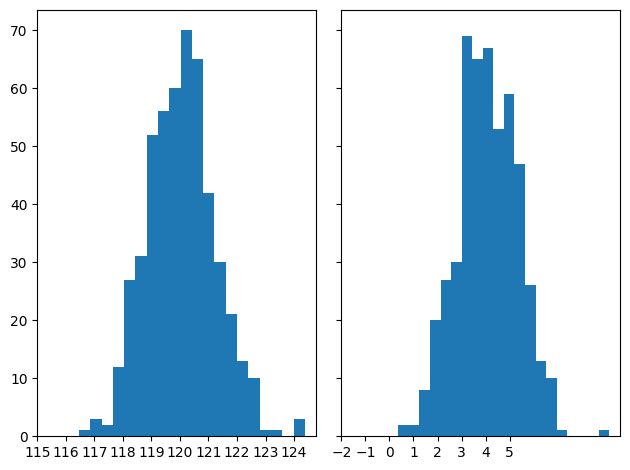
\includegraphics[scale=0.5]{hw0/biv_gaus.png}
    \item    It looks like about 120.5 is the most likely value of $S$ and about 4.2 is the most likely value of $W$. This makes sense, since these are very close to the means of 120.5 and 4.2, the expected values of $S$ and $W$
    \end{enumerate}
    \item Because the distributions' mean changes when $S$ moves, we can say that $W$ is dependent on $S$
    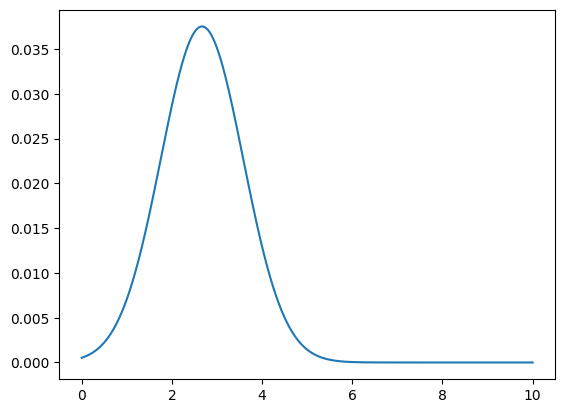
\includegraphics[scale=0.5]{hw0/s118.png}
    \newline
    {$f(W | S = 118)$}
    \newline
    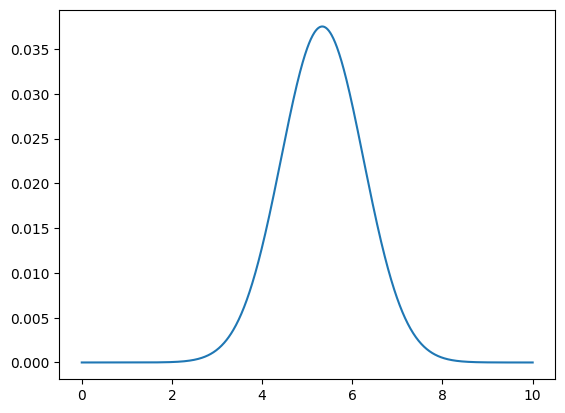
\includegraphics[scale=0.5]{hw0/s122.png}
    \newline
    {$f(W | S = 122)$}
    \item A Gaussian distribution could be a good model for this data because we would expect most packages to fall within a few standard deviation of the mean (i.e., most people will mail packages of a certain size, and not, for example, in a uniform distribution). It might not be a good model because size and weight are not necessarily symmetrically distributed; we might expect that packages would be skewed toward lower numbers, since there would be a few very, very large packages, and some smaller packages. 
    \item $\mathbb{E}(T) = 60 + 0.6\mathbb{E}(W) + 0.2\mathbb{E}(S) + \mathbb{E}(\eps) = 60 + 2.4 + 24 + 0 = 86.4$. For variance, we know $\text{Var}(aX + bY) = a^2 * \text{Var}(X) + b^2 * \text{Var}(Y) + 2ab * \text{Cov}(X, Y)$ in general, so $$\text{Var}(aX + bY) = \text{Var}(0.6W) + \text{Var}(0.2S) + \text{Var}(\eps) + \text{Cov}(W, S) + \text{Cov}(W, \eps) + \text{Cov}(S, \eps)$$
    $$
    = 0.36*1.5 + 0.04*1 + 5 + 1 + 0 + 0 = 0.54 + 0.04 + 6 = 6.58
    $$
    (Since the noise is independent of $W$ and $S$). 
    \item
    \begin{enumerate}
        \item See code.
        \item The mean looks to be around 6200, and the standard deviation looks to be around 500. Indeed, checking our result, the mean is 6201.48 and the standard deviation is 756.73
    \end{enumerate}
\end{enumerate}
\end{document}

